%! Author = Philipp Emmenegger
%! Date = 12/07/2021

\section{Angular}
Flexible SPA Framework for CRUD applications
\begin{itemize}
    \item Typescript 4.1 based
    \item Reduces boilerplate Code
    \item Dependency Injection Mechanism
    \item JS-optimized 2-way binding
    \item Clearly structured, information hiding
    \item Increases testability / maintainability of client-side code
\end{itemize}


\subsection{Architecture}
\textbf{ngModules:} Cohesive block of code dedicated to closely related set of capabilities. (\textit{module})
\textbf{Directives:} Provides instructions to transform the DOM. (\textit{class})
\textbf{Components:} Directive-with-a-template; it controls a section of the view. (\textit{class})
\textbf{Templates:} Form of HTML defining how to render the component. (\textit{HTML / CSS})
\textbf{Metadata:} Describes a class and defines how to process it. (\textit{decorator})
\textbf{Services:} Provides logic of any value, function or feature that the app needs. (\textit{class})

\subsubsection{Angular Modules (ngModule)}
Base for Angular modularity system. Every app has at least one Module, the root Module (a.k.a app).
Root Module ist launched to bootstrap the app.
Modules export features (directives, services) required by other modules.\\
\textbf{TypeScript Module vs. ngModule:}\\
ngModule is a logical block of multipe TypeScript modules linked together.
The ngModule declaration itself is placed into a TypeScript module.
Modules can accommodate sub-modules. All public TS members are exported as an overall \textit{barrel}
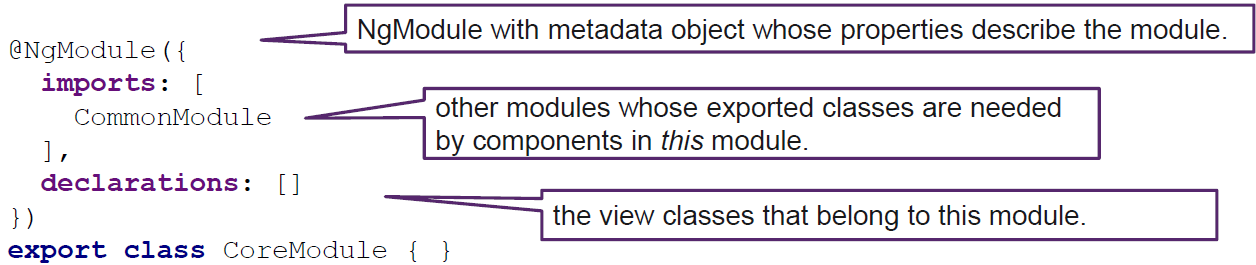
\includegraphics[width=\linewidth]{img/angular_module_declaration.png}
\textit{declarations:} View Classes that belong to this module (Components, Directives, Pipes).\\
\textit{exports:} Subset of declarations that should be visible and usable by other modules.\\
\textit{imports:} Specifies the modules which exports/providers should be imported.\\
\textit{providers:} Creators of services that this module contributes to the global collection of services (DI Container).
They become accessible in all parts of the app.\\
\textit{bootstrap:} Main application view, root component. Only the root module should set this property.

\subsection{Components}
Manages the view and binds data from the model. Consists of:
\begin{itemize}
    \item Controller (App logic), TS Class with \textit{@Component} decorator
    \item HTML file, visual interface (HTML / template expression)
    \item (S)CSS file, styles behind HTML
\end{itemize}
Can be nested, results in Component tree.\\
Provide \textbf{Information Hiding:}
\begin{itemize}
    \item Each Component declares part of the UI
    \item Should be implemented as small coherent piece to support:
    \begin{itemize}
        \item Testability, Maintainability, Reusability
    \end{itemize}
\end{itemize}
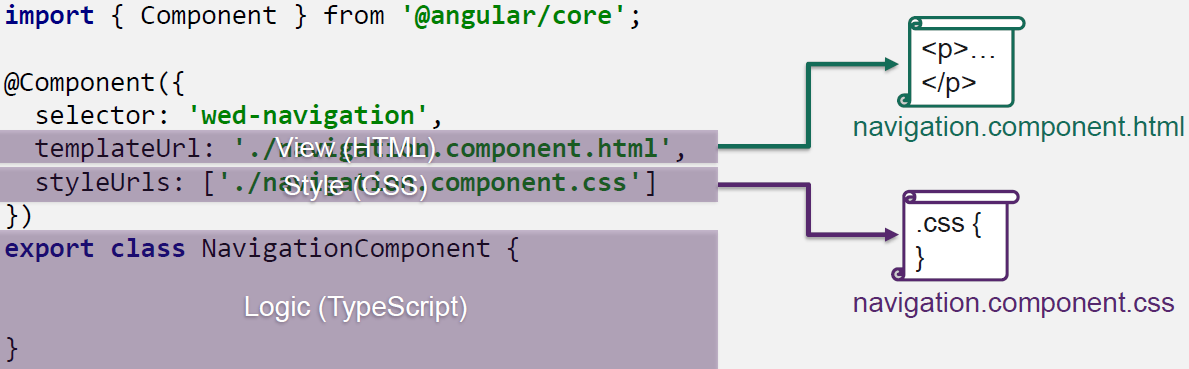
\includegraphics[width=\linewidth]{img/angular_component_declaration.png}
Components must be declared within the containing module so its \textbf{selector} is registered for all sub-components of that module.
They can be exported, so other modules can import and use then.

\subsubsection{Component Lifecycle}
\begingroup
\setlength{\intextsep}{0pt}
\setlength{\columnsep}{20pt}
\begin{wrapfigure}{r}{0.3\linewidth}
    \centering
    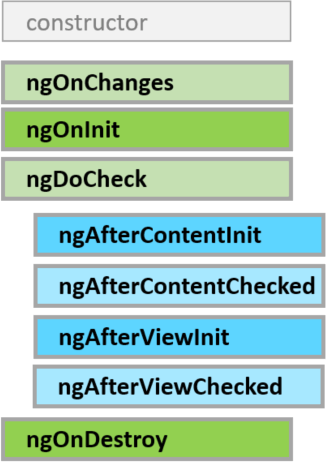
\includegraphics[width=0.7\linewidth]{img/angular_component_lifecycle.png}
\end{wrapfigure}
Most important events are \textbf{ngOnInit} (Creation / Hydration) and \textbf{ngOnDestroy} (Destruction / Dehydration).\\
\textbf{ngAfter...} events are mainly for control developers to handle sub-components and their DOM.
To hook into the lifecycle, interfaces of the Angular core can be implemented.
Each interface has a single hook method, prefixed with \textit{ng}. (\textbf{OnInit} contains method \textit{ngOnInit}).\\
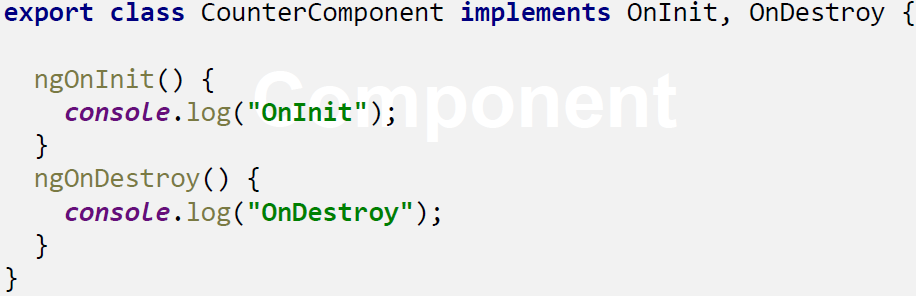
\includegraphics[width=\linewidth]{img/angular_component_lifecycle2.png}

\subsubsection{Content Projection}
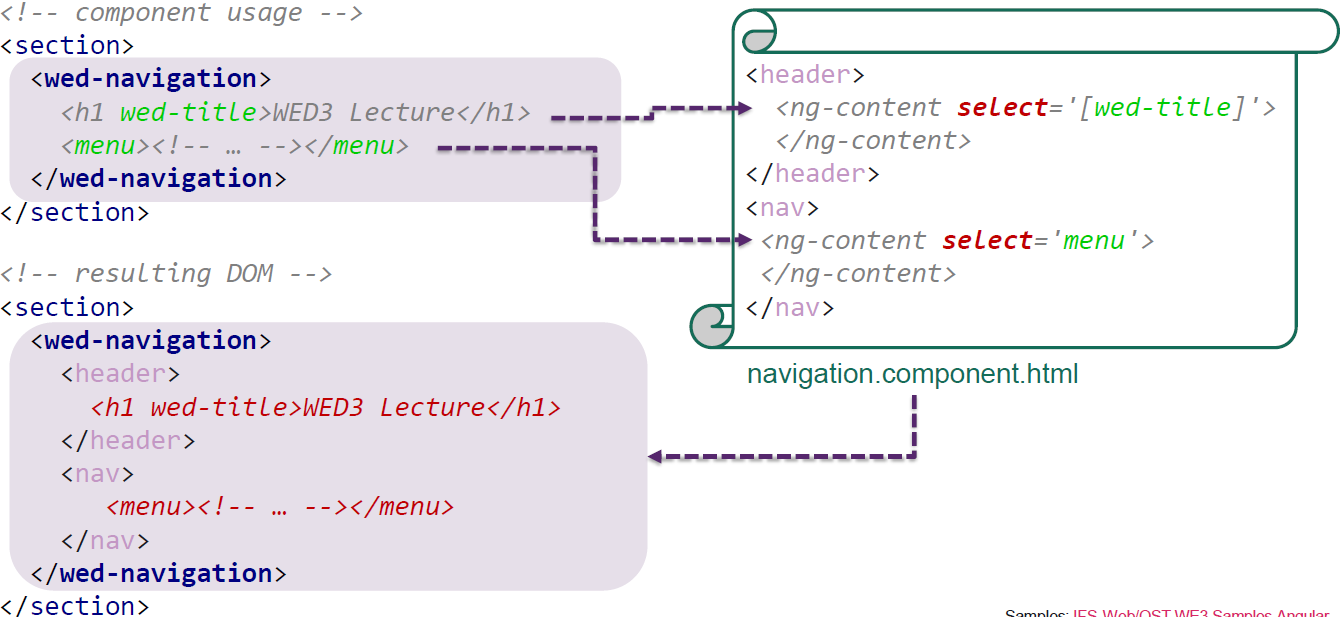
\includegraphics[width=\linewidth]{img/angular_content_projection.png}

\subsection{Templates}
View in MVC.
Written in HTML annotated with Angular \textbf{template syntax}:
\begin{itemize}
    \item HTML5 except script-Tag
    \item Angular extends the HTML with
    \begin{itemize}
        \item Interpolation (\textit{{{...}}})
        \item Template Expression/Statements
        \item Binding Syntax
        \item Directives
        \item Template Reference Variables
        \item Template Expression Operators
    \end{itemize}
\end{itemize}

\subsubsection{Binding}
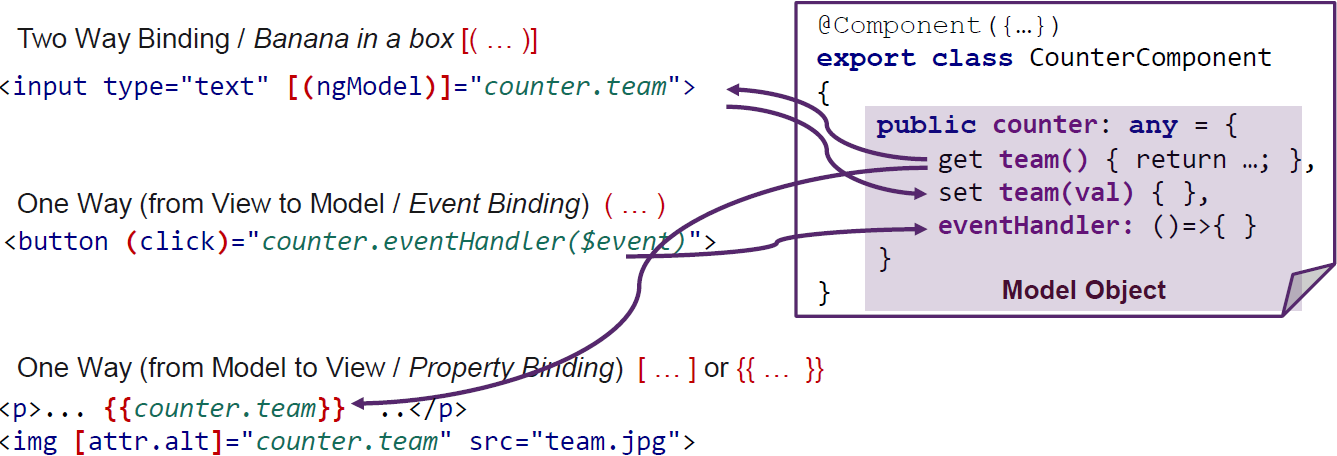
\includegraphics[width=\linewidth]{img/angular_bindings.png}
Binding targets must be declared as \textbf{Inputs or Outputs:} Targets stand on the left side of the binding declaration.
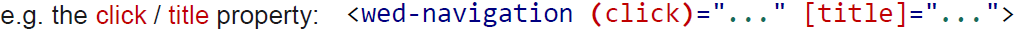
\includegraphics[width=\linewidth]{img/angular_input_output_properties.png}
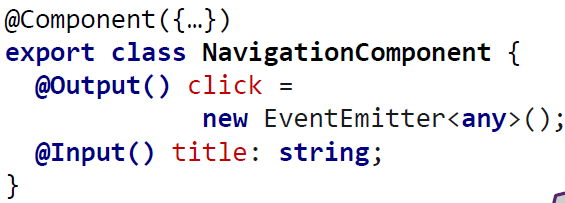
\includegraphics[width=0.5\linewidth]{img/angular_input_output_properties2.png}

\subsection{Directives}
Similar to a component, but without a template.
TypeScript class with an \textit{@Directive()} function decorator.
\subsubsection{Attribute Directives}
Changes the appearance or behaviour of an element, component or another directive.
Applied to a host element as an attribute.
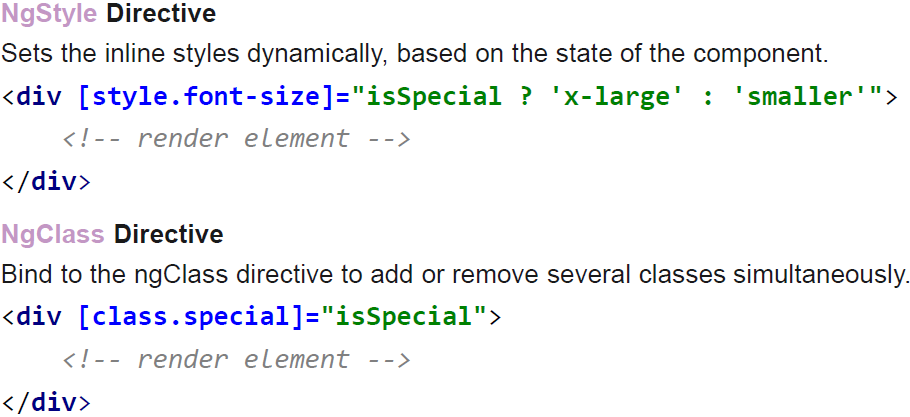
\includegraphics[width=0.6\linewidth]{img/angular_attribute_directives.png}
\subsubsection{Structural Directives}
Responsible for HTML layout.
Reshape the DOM's structure by adding, removing or manipulating elements.
Applied to a host element as an attribute.
Asterisk (*) precedes the directive attribute name.
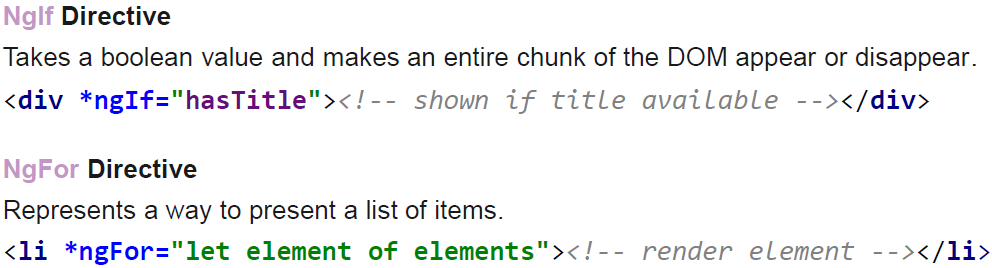
\includegraphics[width=0.6\linewidth]{img/angular_structural_directive.png}
\textbf{NgTemplates:}

\includegraphics[width=0.6\linewidth]{img/angular_ng_templates.png}
Aren't rendered directly.
They need a directive or component which takes over this part.
Can be referenced by their \textit{#id}:\\
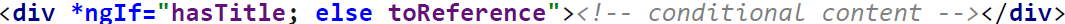
\includegraphics[width=0.8\linewidth]{img/angular_ng_templates2.png}

\subsubsection{Template Reference Variables}
References a DOM element within a template.
Can also be a reference to an component or directive.
A hash (#) declares a reference variable.\\
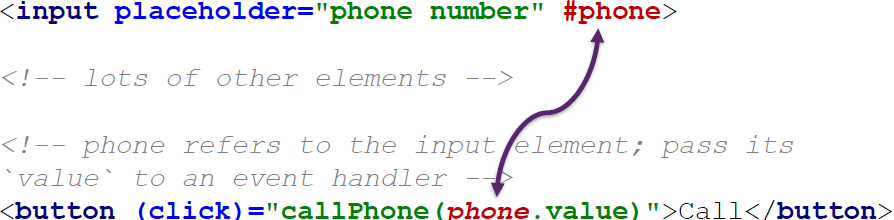
\includegraphics[width=0.7\linewidth]{img/angular_template_reference.png}


\subsection{Services}
Provides any value, function or feature.
Typical Services: logging service, data service, message bus, tax calculator, etc.\\
\textbf{Strongly related to DI:} Angular uses DI to provide components with needed services.
Therefore, services must be registered within the DI container.
\begin{lstlisting}
@Injectable ({ providedIn: 'root' })
export class CounterService { /* ... */ }
\end{lstlisting}
\textit{providedIn: 'root'}: The service is registered for the whole application.
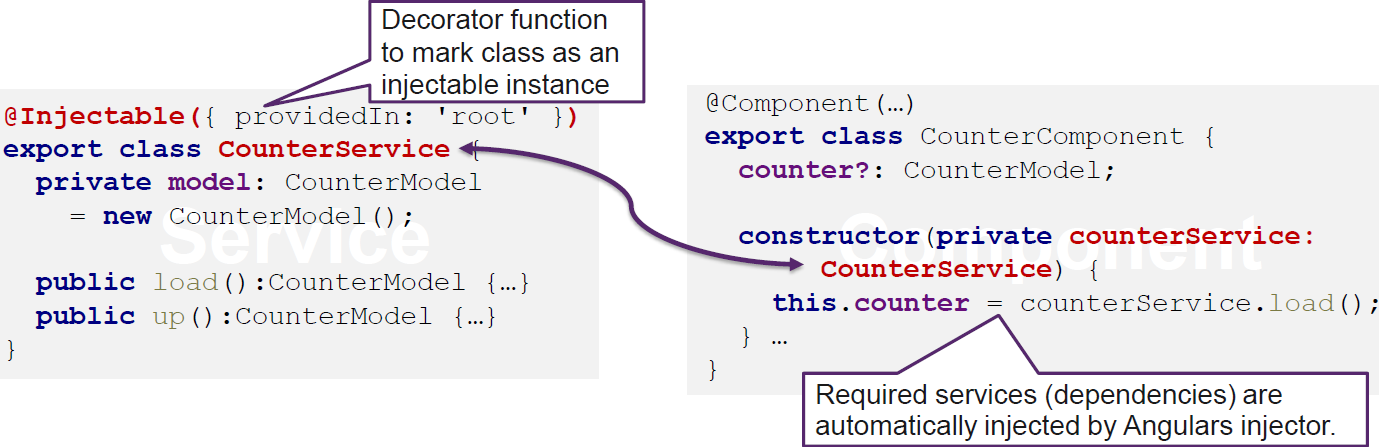
\includegraphics[width=\linewidth]{img/angular_services.png}


\subsection{Forms}
Angular Forms is an external, optional ngModule called FormsModule.
It's a combination of multiple provided services and multiple directives (ngModel, ngForm, ngSubmit).\\
\textbf{Template-driven forms:} Angular Template syntax with the form-specific directives and techniques.
Less code but places validation logic into HTML. (Useful for small forms)\\
\textbf{Reactive / model driven forms:} Import ReactiveFormsModule.
Form is built within the Controller (FormBuilder).
Validation logic is also part of the controller (easier to test).

\subsubsection{Template-driven}
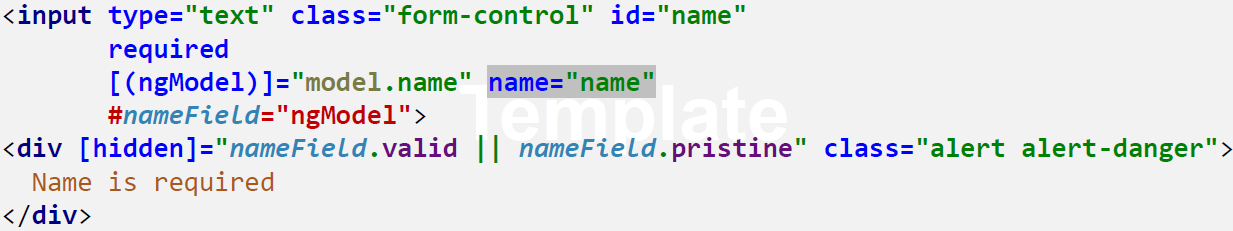
\includegraphics[width=\linewidth]{img/angular_forms.png}
\textbf{Two-Way-Binding:} [(ngModel)] directive to bind values.
Reads out the value of the model for the first time.
Updates are automatically written back into the bound model.\\
\textbf{Validation:} Reference the [ngModel] directive and check its valid property.\\
\textbf{Submitting the form:}\\
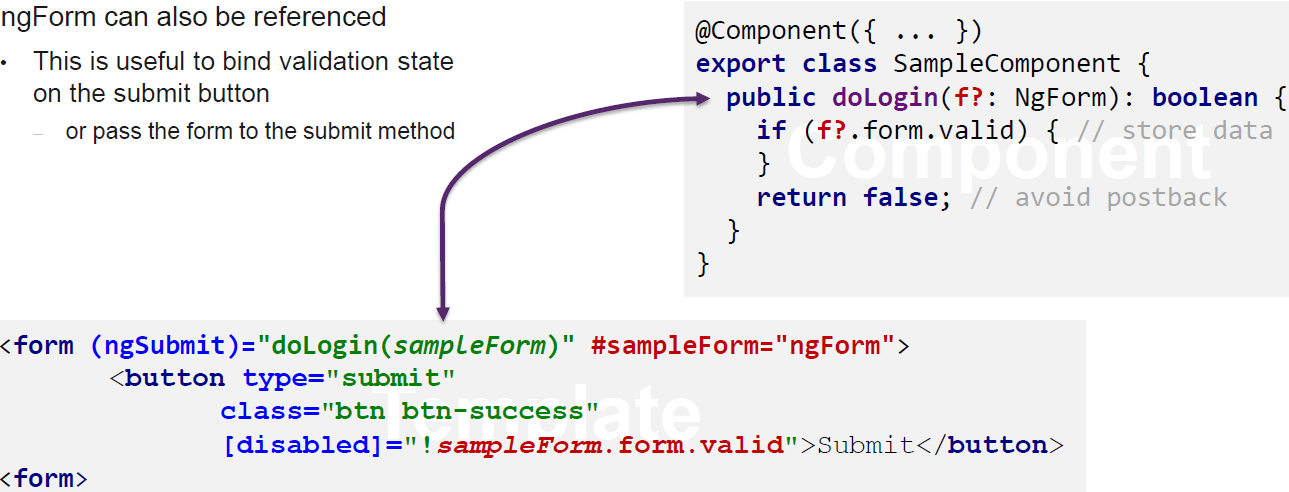
\includegraphics[width=0.8\linewidth]{img/angular_forms_submit.png}


\subsection{Asynchronous Services}
\textbf{Event Emitter example:}\\
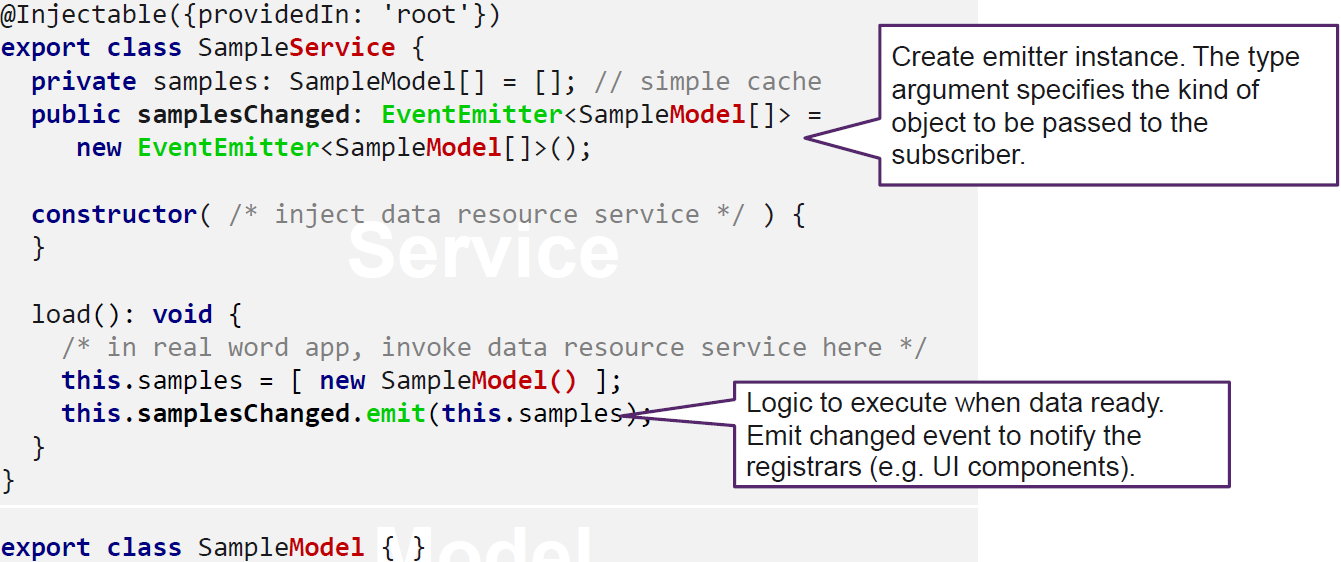
\includegraphics[width=\linewidth]{img/angular_asynchronous_services.png}
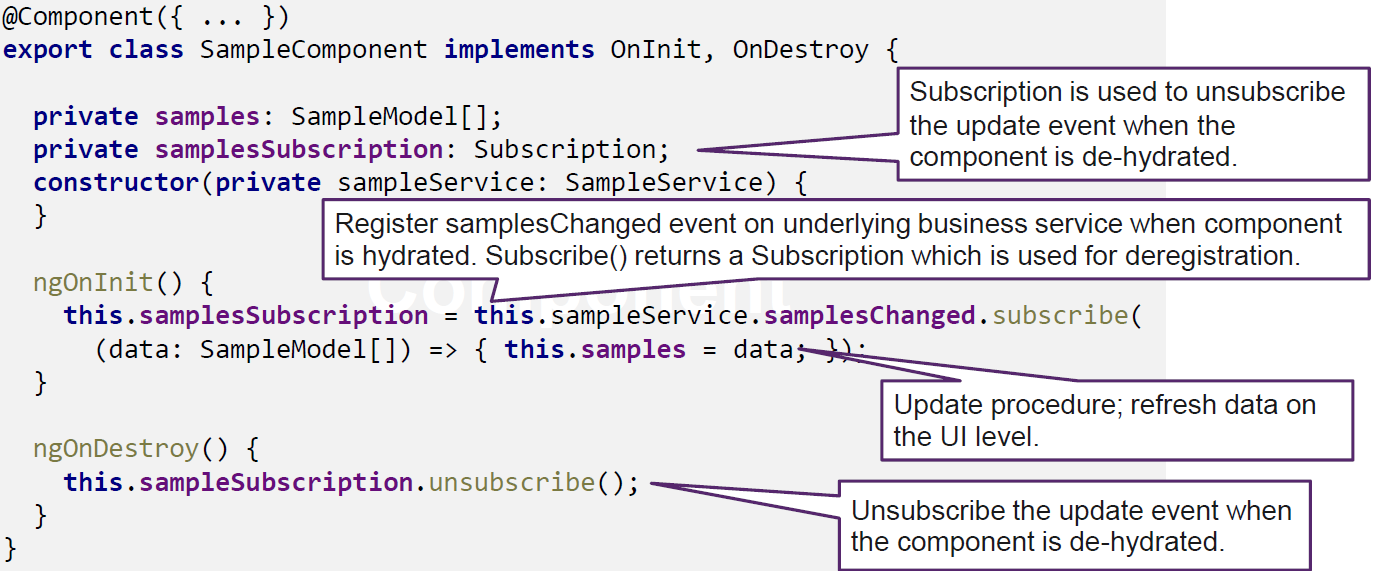
\includegraphics[width=\linewidth]{img/angular_asynchronous_services2.png}

\subsection{Data Access}
\subsubsection{HTTP Client API}
Implements asynchronisms by using the RxJS library.
RxJS is a third-party library that implements the Observable pattern.
An Observable can be turned into a promise.\\
\textbf{Hot Observables:} Sequences of events (mouse moves / stock tickers).
Shared amoung all subscribers.\\
\textbf{Cold Observables:} Start running on subscriptions (such as async web requests).
Not shared amoung subscribers.
Are automatically closed after Task is finished.\\
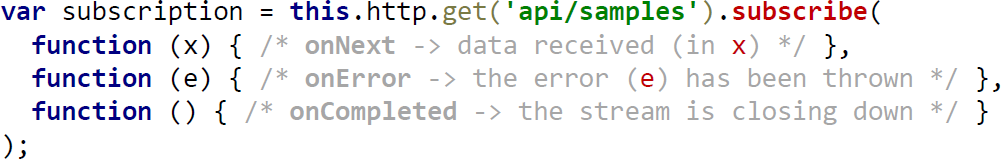
\includegraphics[width=0.8\linewidth]{img/angular_observable.png}


\subsection{Routing}
External, optional NgModule called RouterModule.
Combination of multiple provided services and directives: \textit{RouterOutlet, RouterLink, RouterLinkActive}.\\
\textbf{Defining Routes:} The router must be configured with a list of route definitions.
Each definition maps a route to a component.
\begin{itemize}
    \item \textit{.forRoot():} use exactly once to declare routes on root level
    \item \textit{.forChild():} When declaring sub-routings
\end{itemize}
Each ngModule defines its own routes.
Load modules on-demand (lazy load) with the \textit{import}-Syntax.